\section{Requirements}
\label{sec:eval_requirements} 

Please note that the exact requirement calculation methods are quite complex and will be added at a later point. \\

\subsection{Detection}
\label{sec:eval_req_detection} 

\begin{figure}[H]
    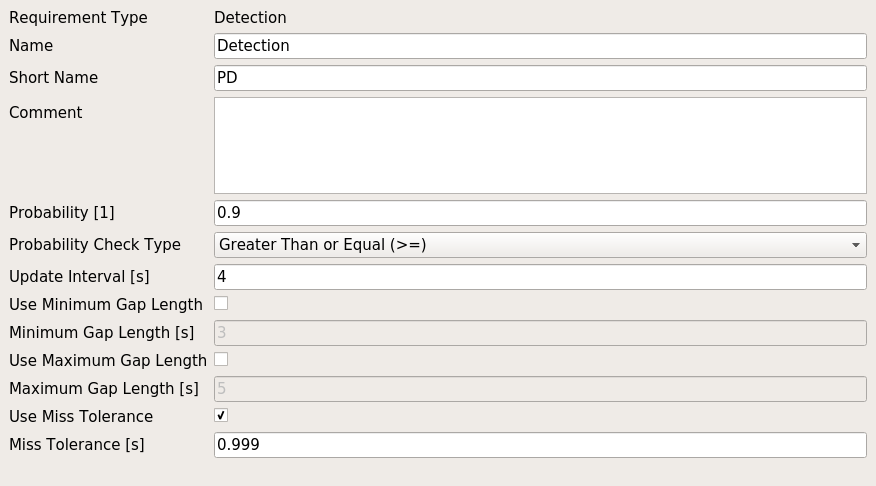
\includegraphics[width=14cm,frame]{../screenshots/eval_req_detection.png}
  \caption{Evaluation Detection requirement}
\end{figure}

The 'Detection' requirement can be used to check whether targets are detected at all. For each target existing in the reference data (within the current sector) a target must be detected within e.g. each test update interval or other given interval. Missed update intervals are either called misses or gaps, which are used to calculate a probability of detection, which has to fulfill a given threshold. \\

\begin{itemize}  
\item Probability [1]: Probability of detection
\item Probability Check Type: $\geq$
\item Update Interval [s]: Update interval of the test data
\item Use Minimum Gap Length: Checkbox if minimum gap length should be used
\item Minimum Gap Length [s]: Minimum gap length to be considered
\item Use Maximum Gap Length: Checkbox if maximum gap length should be used
\item Maximum Gap Length [s]: Maximum gap length to be considered
\item Use Miss Tolerance: Checkbox if miss tolerance should be used
\item Miss Tolerance [s]: Acceptable time delta for miss detection
\end{itemize}
\ \\

As a summary, the reference is used to calculate the number of expected update intervals inside the sector layer (\#EUI). Then, for the test data, if the reference exists at the time, time differences between target reports are checked and the number of misses/gaps are calculated as number of missed update intervals (\#MUI). \\

Gaps are, if a minimum or maximum gap length is used, only counted if the detected gap fulfills the thresholds. \\

The ratio of \#MUI and \#EUI gives the probability of missed update interval, the counter-probability gives the Probability of Detection (PD). The PD must greator or equal than the defined 'Probability' for the requirement to pass.


\subsection{Extra Data}
\label{sec:eval_req_extra_data} 

\begin{figure}[H]
    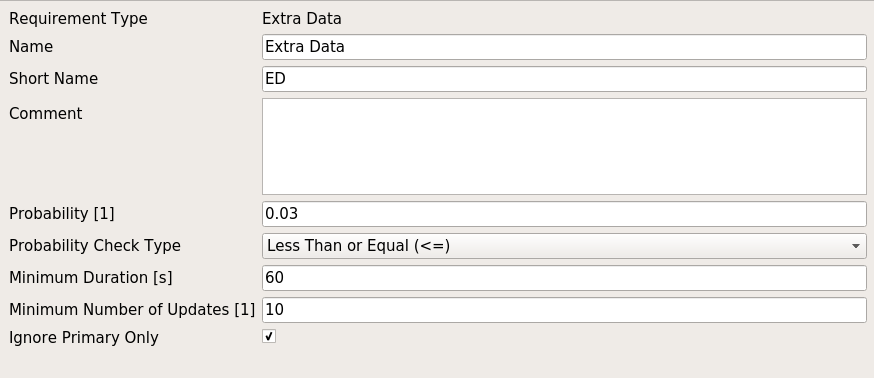
\includegraphics[width=14cm,frame]{../screenshots/eval_req_extra_data.png}
  \caption{Evaluation Extra Data requirement}
\end{figure}

The 'Extra Data' requirement is a recommended addition to the 'Detection' requirement, while not mandated by any standard known to the author. \\

While the 'Detection' requirement detects "missing" test data, it ignores test data for which no reference exist - which might indicate issues in the reference data which might be of interest in the evaluation. \\

The 'Extra Data' requirement detects "extra" test data, i.e. test data for which no reference exists (and fulfills possible constraints), and calculates the number of extra target reports. Based on the number of target reports which are extra, and the number of target reports which are also detection by the reference, the Probability of Extra (PEx) data is calculated. The PEx must be less or equal than the defined 'Probability' for the requirement to pass. \\

\begin{itemize}  
\item Probability [1]: Probability of extra data
\item Probability Check Type: $\leq$
\item Minimum Duration [s]: Minimum track duration, requirement result is ignored if less
\item Minimum Number of Updates [s]: Minimum number of extra target reports, requirement result is ignored if less
\item Ignore Primary Only: Requirement result is ignored if target is primary only (has no secondary attributes, also not in reference)
\end{itemize}
\ \\

\subsection{Extra Track}
\label{sec:eval_req_extra_track} 

\begin{figure}[H]
    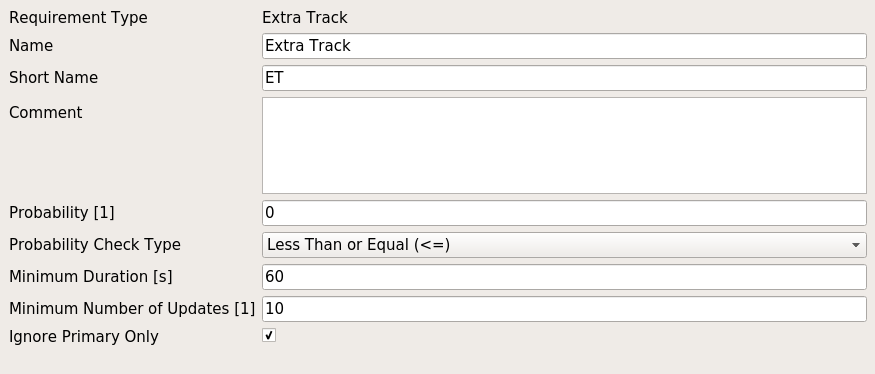
\includegraphics[width=14cm,frame]{../screenshots/eval_req_extra_track.png}
  \caption{Evaluation Extra Track requirement}
\end{figure}

The 'Extra Track' requirement is useful for Tracker evaluation, and detects if more than one test track exist for a target. \\

First the time period of each track (by ocurrance of track number, with a maximum time difference of 5 minutes) is calculated. Then, for each test target report, it is checked if multiple track number periods match, and counted as extra update if there are more than 1. Based on the number of target reports which are extra, and the number of target reports which are also detection by the reference, the Probability of Extra (PEx) data is calculated. The PEx must be less or equal than the defined 'Probability' for the requirement to pass. \\

\begin{itemize}  
\item Probability [1]: Probability of extra data
\item Probability Check Type: $\leq$
\item Minimum Duration [s]: Minimum track duration, requirement result is ignored if less
\item Minimum Number of Updates [s]: Minimum number of extra target reports, requirement result is ignored if less
\item Ignore Primary Only: Requirement result is ignored if target is primary only (has no secondary attributes, also not in reference)
\end{itemize}
\ \\

Please note that currently, in the case of multiple tracks existing at the same time, the requirement does not decided which track is correct and which one is extra, therefore all target reports are counted as being extra. \\

\subsection{Identification Correct}
\label{sec:eval_req_id_correct} 

\begin{figure}[H]
    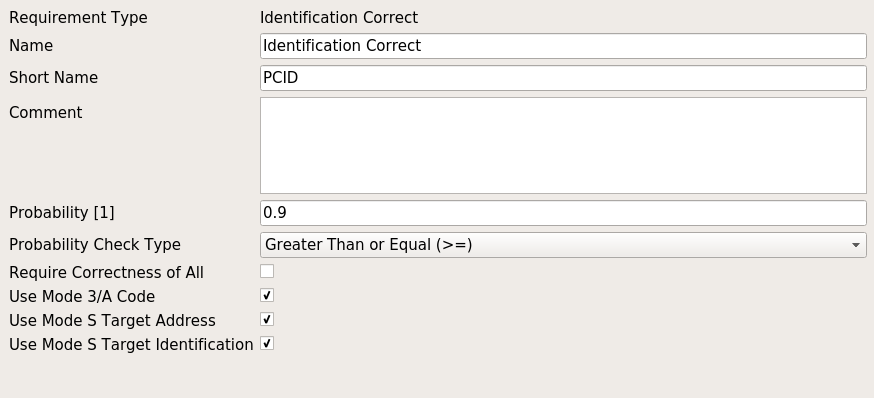
\includegraphics[width=14cm,frame]{../screenshots/eval_req_id_correct.png}
  \caption{Evaluation Identification Correct requirement}
\end{figure}

The 'Identification Correct' requirement is used to calculate the probability of a target report having a correct (secondary) identification. Correct in this context means there is identification data available, and it is the same as in the reference. \\

\begin{itemize}  
\item Probability [1]: Probability of correct identification
\item Probability Check Type: $\geq$
\item Require correctness of All: If checked, all available secondary attributes must match the reference. If not checked, a single matching secondary attribute is enough.
\item Use Mode 3/A Code: If the Mode 3/A code should be checked
\item Use Mode S Target Address: If the Mode S target address should be checked
\item Use Mode S Target Identification: If the Mode S target identification should be checked
\end{itemize}
\ \\

\subsection{Identification False}
\label{sec:eval_req_id_false} 

\begin{figure}[H]
    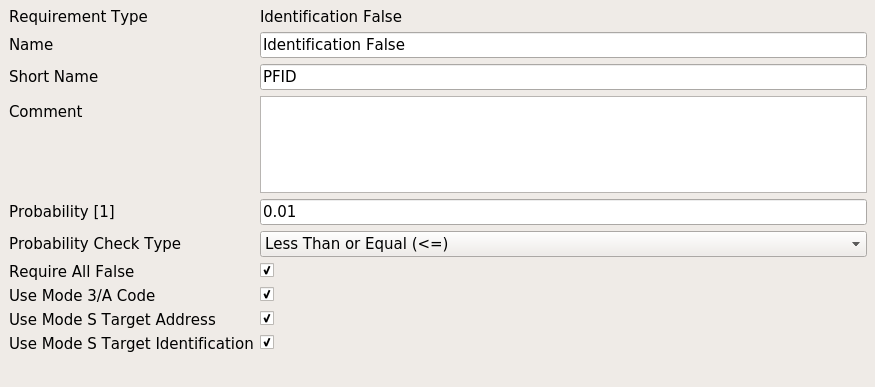
\includegraphics[width=14cm,frame]{../screenshots/eval_req_id_false.png}
  \caption{Evaluation Identification False requirement}
\end{figure}

The 'Identification False' requirement is used to calculate the probability of a target report having a false (secondary) identification. False in this context means there is identification data available, and it is not the same as in the reference. \\

\begin{itemize}  
\item Probability [1]: Probability of false identification
\item Probability Check Type: $\leq$
\item Require All False: If checked, all available secondary attributes be different than in the reference to count. If not checked, a single wrong secondary attribute is enough.
\item Use Mode 3/A Code: If the Mode 3/A code should be checked
\item Use Mode S Target Address: If the Mode S target address should be checked
\item Use Mode S Target Identification: If the Mode S target identification should be checked
\end{itemize}
\ \\

\subsection{Mode 3/A False}
\label{sec:eval_req_m3a_false} 

\begin{figure}[H]
    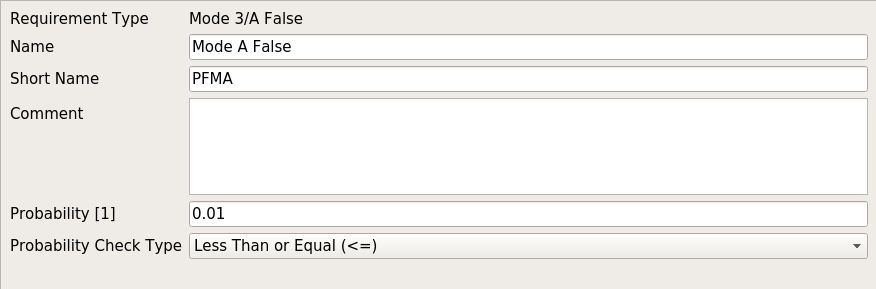
\includegraphics[width=14cm,frame]{../screenshots/eval_req_m3a_false.png}
  \caption{Evaluation Mode 3/A False requirement}
\end{figure}

The 'Mode 3/A False' requirement is used to calculate the probability of a target report having a false Mode 3/A code. False in this context means there is Mode 3/A information data available, and it is not the same as in the reference. \\

\begin{itemize}  
\item Probability [1]: Probability of false Mode 3/A code
\item Probability Check Type: $\leq$
\end{itemize}
\ \\

\subsection{Mode 3/A Present}
\label{sec:eval_req_m3a_present} 

\begin{figure}[H]
    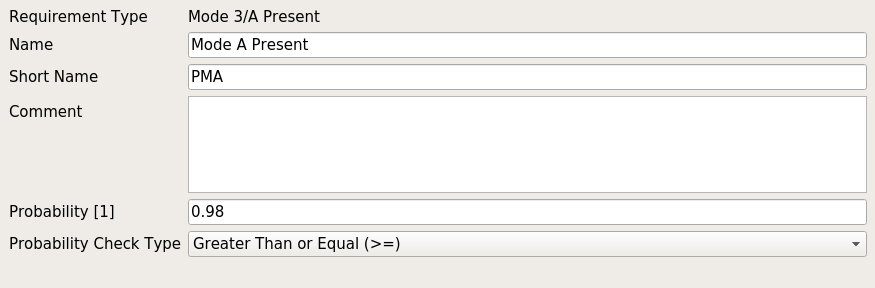
\includegraphics[width=14cm,frame]{../screenshots/eval_req_m3a_present.png}
  \caption{Evaluation Mode 3/A Present requirement}
\end{figure}

The 'Mode 3/A Present' requirement is used to calculate the probability of a target report having any Mode 3/A code. Present in this context means there is Mode 3/A information data available, irrespectively if correct or not. \\

\begin{itemize}  
\item Probability [1]: Probability of Mode 3/A code present
\item Probability Check Type: $\geq$
\end{itemize}
\ \\

\subsection{Mode C False}
\label{sec:eval_req_mc_false} 

\begin{figure}[H]
    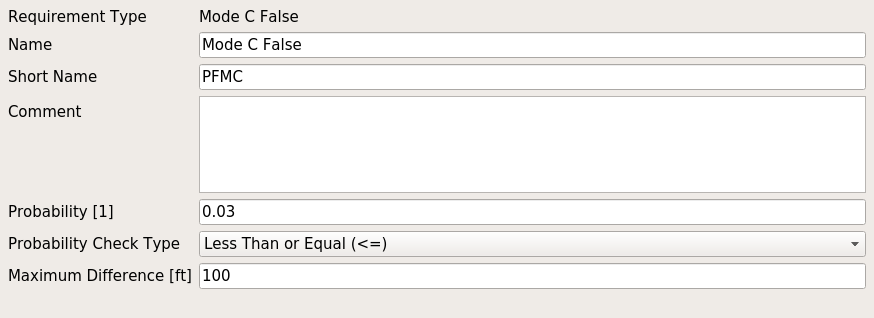
\includegraphics[width=14cm,frame]{../screenshots/eval_req_mc_false.png}
  \caption{Evaluation Mode C False requirement}
\end{figure}

The 'Mode C False' requirement is used to calculate the probability of a target report having a false Mode C code. False in this context means there is Mode C information data available, and the absolute difference between the test and the reference is larger than the given threshold. \\

\begin{itemize}  
\item Probability [1]: Probability of false Mode C code
\item Probability Check Type: $\leq$
\item Maximum Difference [ft]: Maximum altitude difference between the test and the reference, in feet
\end{itemize}
\ \\

\subsection{Mode C Present}
\label{sec:eval_req_mc_present} 

\begin{figure}[H]
    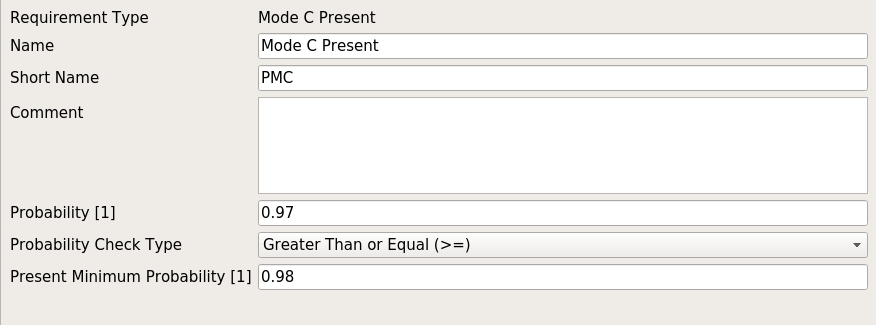
\includegraphics[width=14cm,frame]{../screenshots/eval_req_mc_present.png}
  \caption{Evaluation Mode C Present requirement}
\end{figure}

The 'Mode C Present' requirement is used to calculate the probability of a target report having any Mode C code. Present in this context means there is Mode C information data available, irrespectively if correct or not. \\

\begin{itemize}  
\item Probability [1]: Probability of Mode C code present
\item Probability Check Type: $\geq$
\end{itemize}
\ \\

\subsection{Position Across}
\label{sec:eval_req_pos_across} 

\begin{figure}[H]
    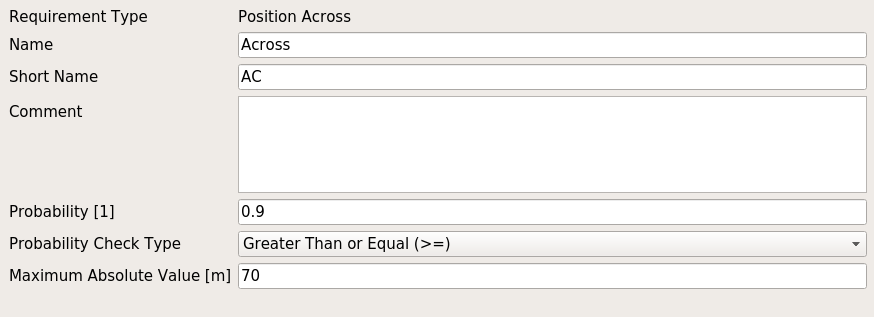
\includegraphics[width=14cm,frame]{../screenshots/eval_req_pos_across.png}
  \caption{Evaluation Position Across requirement}
\end{figure}

The 'Position Across' requirement is used to calculate the probability of a target report having an across-track error smaller than a defined threshold. The offset of the position (test vs. linear interpolated reference position) is used to calculate the error component across the track angle of the reference at the time. If the absolute value of this across-track position error is smaller or equal than the defined threshold, the target report is counted for the calculated probability PACOK. The PACOK must be greater or equal than the defined 'Probability' for the requirement to pass.

\begin{itemize}  
\item Probability [1]: Probability of false Mode C code
\item Probability Check Type: $\geq$
\item Maximum Absolute Value [m]: Maximum absolute across-track position difference between the test and the reference, in meters
\end{itemize}
\ \\

\subsection{Position Along}
\label{sec:eval_req_pos_along} 

\begin{figure}[H]
    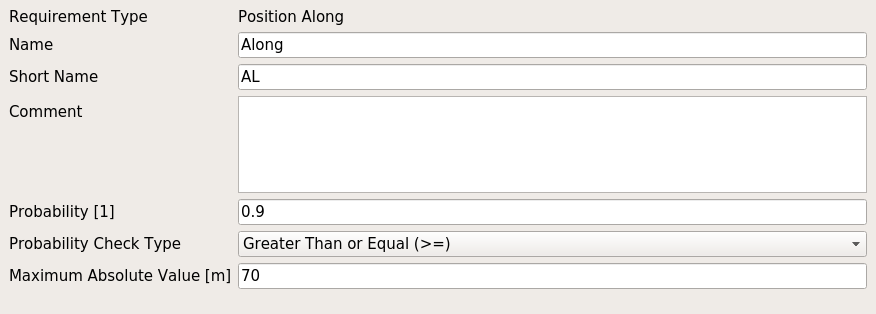
\includegraphics[width=14cm,frame]{../screenshots/eval_req_pos_along.png}
  \caption{Evaluation Position Along requirement}
\end{figure}

The 'Position Along' requirement is used to calculate the probability of a target report having an along-track error smaller than a defined threshold. The offset of the position (test vs. linear interpolated reference position) is used to calculate the error component along the track angle of the reference at the time. If the absolute value of this along-track position error is smaller or equal than the defined threshold, the target report is counted for the calculated probability PALOK. The PALOK must be greater or equal than the defined 'Probability' for the requirement to pass.

\begin{itemize}  
\item Probability [1]: Probability of false Mode C code
\item Probability Check Type: $\geq$
\item Maximum Absolute Value [m]: Maximum absolute along-track position difference between the test and the reference, in meters
\end{itemize}
\ \\

\subsection{Position Distance}
\label{sec:eval_req_pos_distance} 

This requirement can be used in 2 variations:

\begin{figure}[H]
    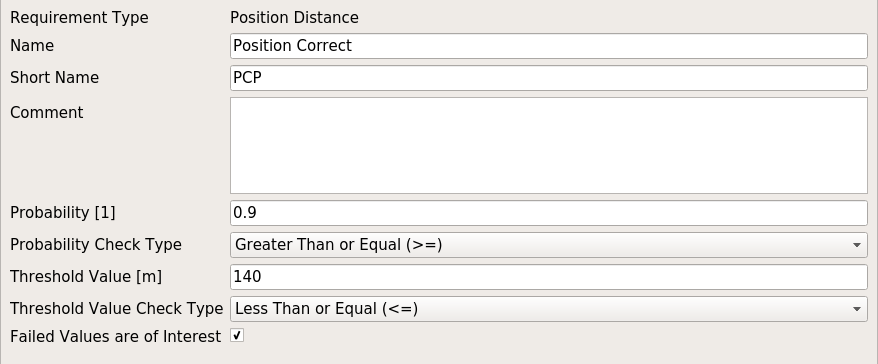
\includegraphics[width=14cm,frame]{../screenshots/eval_req_pos_distance_correct.png}
  \caption{Evaluation Position Distance requirement for correct positions}
\end{figure}

\begin{figure}[H]
    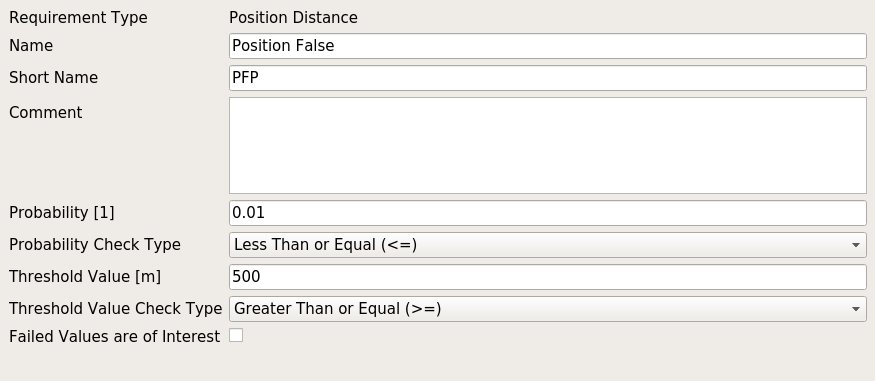
\includegraphics[width=14cm,frame]{../screenshots/eval_req_pos_distance_false.png}
  \caption{Evaluation Position Distance requirement for false positions}
\end{figure}

The 'Position Distance' requirement is used to calculate the probability of a target report having a position error smaller or larger than a defined threshold. This two possibilities allow for calculation of a position correct or being false (e.g. outside an $5\sigma$ range of an expected error distribution). \\

The offset of the position (test vs. linear interpolated reference position) is used to calculate the Euklidian error distance. If the  value of this position error is fails the defined comparison threshold, the target report is counted for the calculated probability PCP (probability of check passed). The PCP must be in turn pass the check for the requirement to pass. \\

The 'Failed Values are of Interest' checkbox define if the target reports passing or failing the check are of interest.


\subsection{Position Correct Variation}

\begin{itemize}  
\item Probability [1]: Probability of correct position
\item Probability Check Type: $\geq$
\item Threshold Value [m]: Maximum allowed distance from test target report to reference
\item Threshold Value Check Type: $\leq$, distance must be less or equal the given threshold
\item Failed Values are of Interest: Checked, the distances of interest are the ones not passing the check
\end{itemize}
\ \\

\subsection{Position False Variation}

\begin{itemize}  
\item Probability [1]: Probability of false position
\item Probability Check Type: $\leq$
\item Threshold Value [m]: Minimum distance from test target report to reference
\item Threshold Value Check Type: $\geq$, distance must be greater or equal the given threshold
\item Failed Values are of Interest: Not checked, the distances of interest are the ones passing the check
\end{itemize}
\ \\

\subsection{Position Latency}
\label{sec:eval_req_pos_latency} 

\begin{figure}[H]
    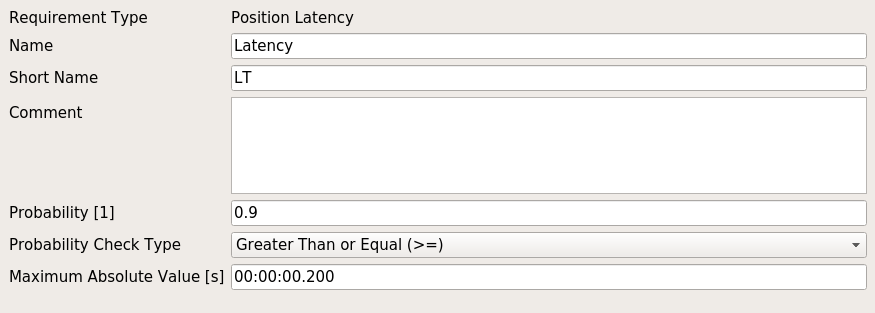
\includegraphics[width=14cm,frame]{../screenshots/eval_req_pos_latency.png}
  \caption{Evaluation Position Latency requirement}
\end{figure}

The 'Position Latency' requirement is used to calculate the probability of a target report having a time-lantency error smaller than a defined threshold. The offset of the position (test vs. linear interpolated reference position) is used to calculate the error component along the track angle of the reference at the time, which divided by the negative speed gives the latency. If the absolute value of this latency is smaller or equal than the defined threshold, the target report is counted for the calculated probability PLTOK. The PLTOK must be greater or equal than the defined 'Probability' for the requirement to pass.

\begin{itemize}  
\item Probability [1]: Probability of false Mode C code
\item Probability Check Type: $\geq$
\item Maximum Absolute Value [s]: Maximum absolute latency, in seconds
\end{itemize}
\ \\

\subsection{Speed}
\label{sec:eval_req_speed} 

\begin{figure}[H]
    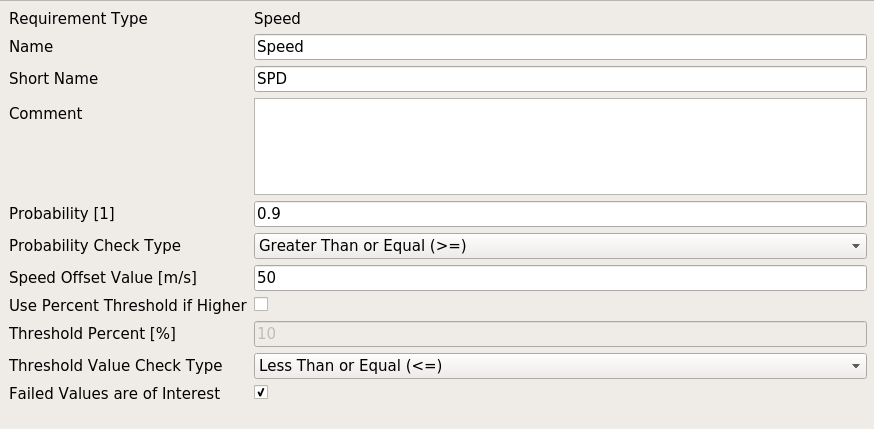
\includegraphics[width=14cm,frame]{../screenshots/eval_req_speed.png}
  \caption{Evaluation Speed requirement}
\end{figure}

The 'Speed' requirement is used to calculate the probability of a target report having an speed error smaller than a defined threshold. The difference of the speed (test speed vs. speed based on reference positions) is calculated, and if its absolute value is smaller or equal than the defined threshold, the target report is counted for the calculated probability PCP (probability of check passed). The PCP must be greater or equal than the defined 'Probability' for the requirement to pass. \\

In another variation, if the 'Use Percent Threshold if Higher' checkbox is set, the check is changed for faster speeds. If the 'Threshold Percent' value times the calculated speed is larger or equal the dewfined threshold value, then threshold value is changed to value of the 'Threshold Percent' value times the calculated speed. This means that for higher speeds, an accuracy with the given percentage is required.

\begin{itemize}  
\item Probability [1]: Probability of false Mode C code
\item Probability Check Type: $\geq$
\item Speed Offset Value [m/s]: Maximum absolute speed difference between the test and the reference, in meters per second
\item Use Percent Threshold if Higher: Defines if the percent-based accuracy should be used for higher speeds
\item Threshold Percent [\%]: Percent threshold
\item Threshold Value Check Type: $\leq$, speed difference must be less or equal the given threshold
\item Failed Values are of Interest: Checked, the speed values of interest are the ones not passing the check
\end{itemize}
\ \\

